\documentclass[11pt,a4paper]{report}
\usepackage[textwidth=37em,vmargin=30mm]{geometry}
\usepackage{calc,xunicode,amsmath,amssymb,paralist,enumitem,tabu,booktabs,datetime2,xeCJK,xeCJKfntef,listings}
\usepackage{tocloft,fancyhdr,tcolorbox,xcolor,graphicx,eso-pic,xltxtra,xelatexemoji}

\newcommand{\envyear}[0]{2025}
\newcommand{\envdatestr}[0]{2025-05-25}
\newcommand{\envfinaldir}[0]{webdb/2025/20250525/final}

\usepackage[hidelinks]{hyperref}
\hypersetup{
    colorlinks=false,
    pdfpagemode=FullScreen,
    pdftitle={Web Digest - \envdatestr}
}

\setlength{\cftbeforechapskip}{10pt}
\renewcommand{\cftchapfont}{\rmfamily\bfseries\large\raggedright}
\setlength{\cftbeforesecskip}{2pt}
\renewcommand{\cftsecfont}{\sffamily\small\raggedright}

\setdefaultleftmargin{2em}{2em}{1em}{1em}{1em}{1em}

\usepackage{xeCJK,xeCJKfntef}
\xeCJKsetup{PunctStyle=plain,RubberPunctSkip=false,CJKglue=\strut\hskip 0pt plus 0.1em minus 0.05em,CJKecglue=\strut\hskip 0.22em plus 0.2em}
\XeTeXlinebreaklocale "zh"
\XeTeXlinebreakskip = 0pt


\setmainfont{Brygada 1918}
\setromanfont{Brygada 1918}
\setsansfont{IBM Plex Sans}
\setmonofont{JetBrains Mono NL}
\setCJKmainfont{Noto Serif CJK SC}
\setCJKromanfont{Noto Serif CJK SC}
\setCJKsansfont{Noto Sans CJK SC}
\setCJKmonofont{Noto Sans CJK SC}

\setlength{\parindent}{0pt}
\setlength{\parskip}{8pt}
\linespread{1.15}

\lstset{
	basicstyle=\ttfamily\footnotesize,
	numbersep=5pt,
	backgroundcolor=\color{black!5},
	showspaces=false,
	showstringspaces=false,
	showtabs=false,
	tabsize=2,
	captionpos=b,
	breaklines=true,
	breakatwhitespace=true,
	breakautoindent=true,
	linewidth=\textwidth
}






\newcommand{\coverpic}[2]{
    % argv: itemurl, authorname
    Cover photo by #2~~(\href{#1}{#1})
}
\newcommand{\makeheader}[0]{
    \begin{titlepage}
        % \newgeometry{hmargin=15mm,tmargin=21mm,bmargin=12mm}
        \begin{center}
            
            \rmfamily\scshape
            \fontspec{BaskervilleF}
            \fontspec{Old Standard}
            \fontsize{59pt}{70pt}\selectfont
            WEB\hfill DIGEST
            
            \vfill
            % \vskip 30pt
            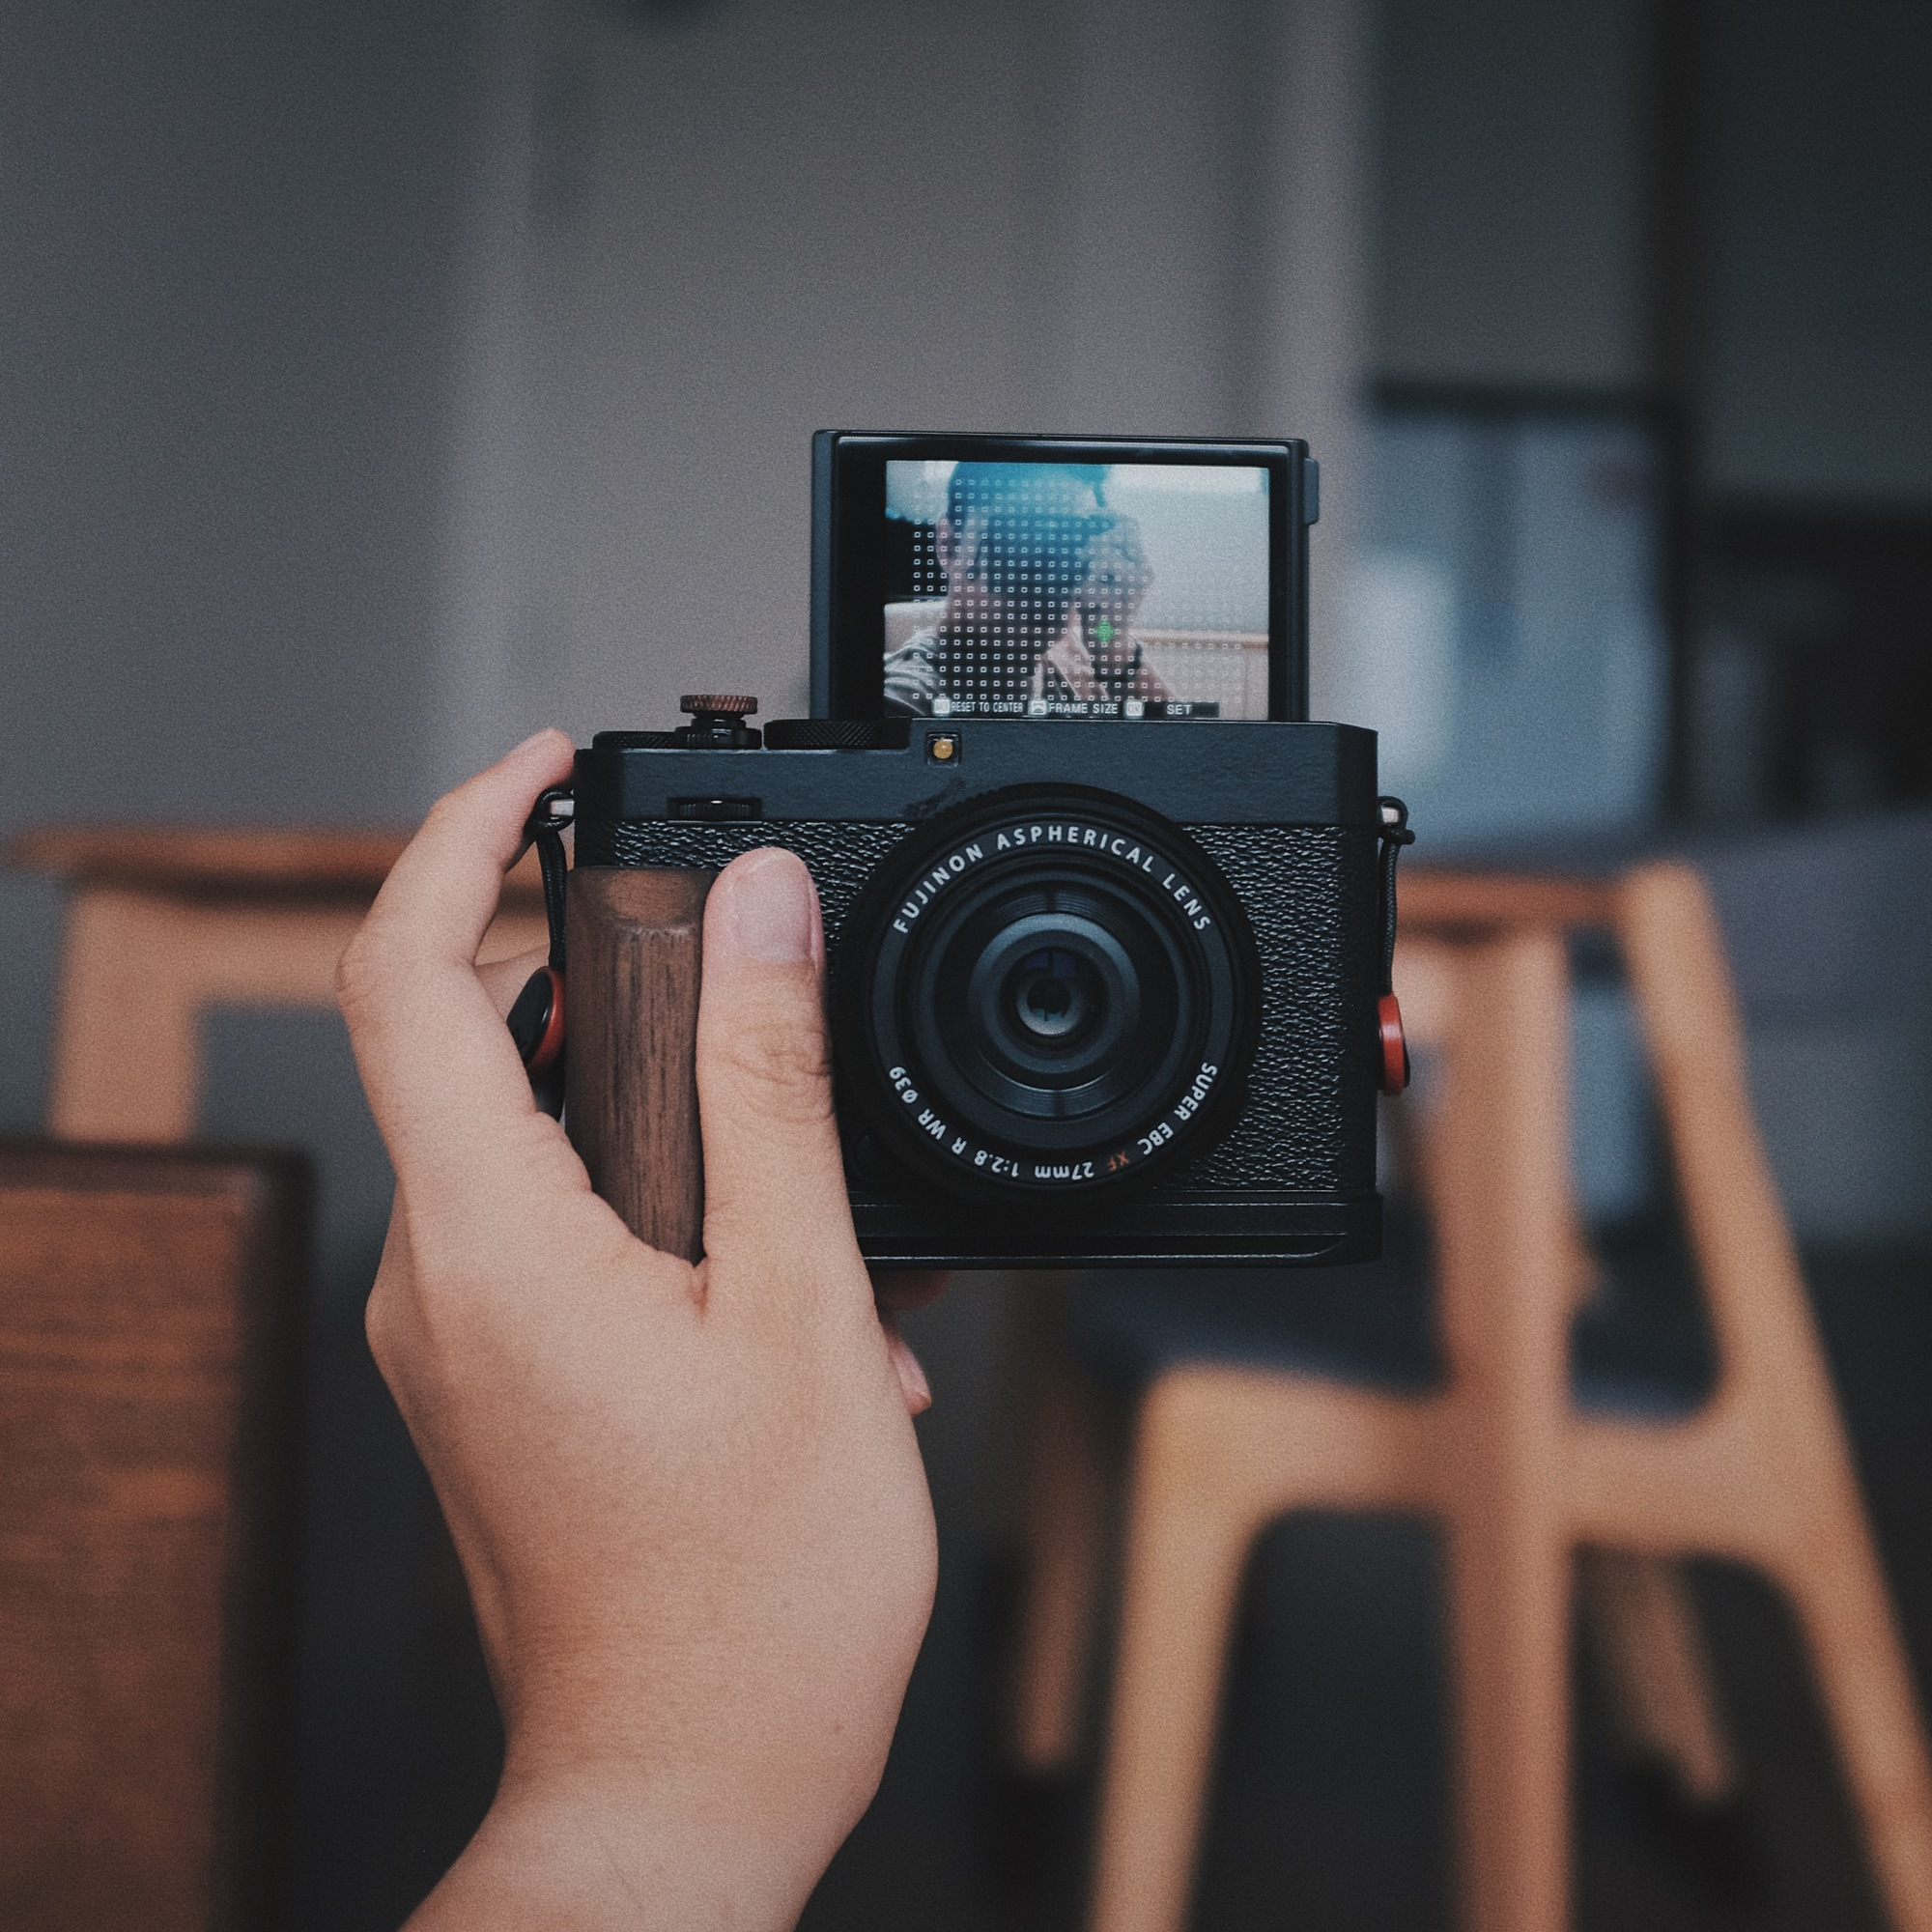
\includegraphics[width=\linewidth]{\envfinaldir/coverpic-prod.jpg}\par
            % \vskip 30pt
            \vfill

            \normalsize\rmfamily\scshape
            \copyright{} The Web Digest Project \hfill\large \envdatestr
        \end{center}
    \end{titlepage}
    % \restoregeometry
}
\newcommand{\simplehref}[1]{%
    \textcolor{blue!80!green}{\href{#1}{#1}}%
}
\renewcommand{\contentsname}{\center\Huge\sffamily\bfseries Contents\par\vskip 20pt}
\newcounter{ipartcounter}
\setcounter{ipartcounter}{0}
\newcommand{\ipart}[1]{
    % \vskip 20pt
    \clearpage
    \stepcounter{ipartcounter}
    \phantomsection
    \addcontentsline{toc}{chapter}{#1}
    % \begin{center}
    %     \Huge
    %     \sffamily\bfseries
    %     #1
    % \end{center}
    % \vskip 20pt plus 7pt
}
\newcounter{ichaptercounter}
\setcounter{ichaptercounter}{0}
\newcommand{\ichapter}[1]{
    % \vskip 20pt
    \clearpage
    \stepcounter{ichaptercounter}
    \phantomsection
    \addcontentsline{toc}{section}{\numberline{\arabic{ichaptercounter}}#1}
    \begin{center}
        \Huge
        \sffamily\bfseries
        #1
    \end{center}
    \vskip 20pt plus 7pt
}
\newcommand{\entrytitlefont}[1]{\subsection*{\raggedright\Large\sffamily\bfseries#1}}
\newcommand{\entryitemGeneric}[2]{
    % argv: title, url
    \parbox{\linewidth}{
        \entrytitlefont{#1}\par\vskip 5pt
        \footnotesize\ttfamily\mdseries
        \simplehref{#2}
    }\vskip 11pt plus 11pt minus 1pt
}
\newcommand{\entryitemGithub}[3]{
    % argv: title, url, desc
    \parbox{\linewidth}{
        \entrytitlefont{#1}\par\vskip 5pt
        \footnotesize\ttfamily\mdseries
        \simplehref{#2}\par\vskip 5pt
        \small\rmfamily\mdseries#3
    }\vskip 11pt plus 11pt minus 1pt
}
\newcommand{\entryitemAp}[3]{
    % argv: title, url, desc
    \parbox{\linewidth}{
        \entrytitlefont{#1}\par\vskip 5pt
        \footnotesize\ttfamily\mdseries
        \simplehref{#2}\par\vskip 5pt
        \small\rmfamily\mdseries#3
    }\vskip 11pt plus 11pt minus 1pt
}
\newcommand{\entryitemHackernews}[3]{
    % argv: title, hnurl, rawurl
    % \parbox{\linewidth}{
    %     \entrytitlefont{#1}\par\vskip 5pt
    %     \footnotesize\ttfamily\mdseries
    %     \simplehref{#3}\par
    %     \textcolor{black!50}{\href{#2}{#2}}
    % }\vskip 11pt plus 11pt minus 1pt
    \begin{minipage}{\linewidth}
            \entrytitlefont{#1}\par\vskip 5pt
            \footnotesize\ttfamily\mdseries
            \simplehref{#3}\par
            \textcolor{black!50}{\href{#2}{#2}}
    \end{minipage}\par\vskip 11pt plus 11pt minus 1pt
}







\begin{document}

\makeheader

\tableofcontents\clearpage




\ipart{Developers}
\ichapter{Hacker News}
\entryitemTwoLinks{Reinvent the Wheel}{https://news.ycombinator.com/item?id=44083467}{https://endler.dev/2025/reinvent-the-wheel/}

\entryitemTwoLinks{Tachy0n: The Last 0day Jailbreak}{https://news.ycombinator.com/item?id=44083388}{https://blog.siguza.net/tachy0n/}

\entryitemTwoLinks{Live facial recognition cameras may become 'commonplace' as police use soars}{https://news.ycombinator.com/item?id=44082326}{https://www.theguardian.com/technology/2025/may/24/police-live-facial-recognition-cameras-england-and-wales}

\entryitemTwoLinks{Good Writing}{https://news.ycombinator.com/item?id=44081586}{https://paulgraham.com/goodwriting.html}

\entryitemTwoLinks{You're a little company, now act like one}{https://news.ycombinator.com/item?id=44081494}{https://longform.asmartbear.com/little-company/}

\entryitemTwoLinks{AI, Heidegger, and Evangelion}{https://news.ycombinator.com/item?id=44081346}{https://fakepixels.substack.com/p/ai-heidegger-and-evangelion}

\entryitemTwoLinks{I used o3 to find a remote zeroday in the Linux SMB implementation}{https://news.ycombinator.com/item?id=44081338}{https://sean.heelan.io/2025/05/22/how-i-used-o3-to-find-cve-2025-37899-a-remote-zeroday-vulnerability-in-the-linux-kernels-smb-implementation/}

\entryitemTwoLinks{Show HN: Rotary Phone Dial Linux Kernel Driver}{https://news.ycombinator.com/item?id=44080803}{https://gitlab.com/sephalon/rotary\_dial\_kmod}

\entryitemTwoLinks{Hong Kong's Famous Bamboo Scaffolding Hangs on (For Now)}{https://news.ycombinator.com/item?id=44080549}{https://www.nytimes.com/2025/05/24/world/asia/hongkong-bamboo-scaffolding.html}

\entryitemTwoLinks{The Xenon Death Flash: How a Camera Nearly Killed the Raspberry Pi 2}{https://news.ycombinator.com/item?id=44080533}{https://magnus919.com/2025/05/the-xenon-death-flash-how-a-camera-nearly-killed-the-raspberry-pi-2/}

\entryitemTwoLinks{DumPy: NumPy except it's OK if you're dum}{https://news.ycombinator.com/item?id=44080181}{https://dynomight.net/dumpy/}

\entryitemTwoLinks{Ask HN: Go deep into AI/LLMs or just use them as tools?}{https://news.ycombinator.com/item?id=44079303}{https://news.ycombinator.com/item?id=44079303}

\entryitemTwoLinks{Valve takes another step toward making SteamOS a true Windows competitor}{https://news.ycombinator.com/item?id=44078930}{https://arstechnica.com/gaming/2025/05/valve-adds-steamos-compatible-game-label-as-it-prepares-to-expand-beyond-steam-deck/}

\entryitemTwoLinks{How to Make a Living as a Writer}{https://news.ycombinator.com/item?id=44078813}{https://thewalrus.ca/how-to-make-a-living-as-a-writer/}

\entryitemTwoLinks{Why Algebraic Effects?}{https://news.ycombinator.com/item?id=44078434}{https://antelang.org/blog/why\_effects/}

\entryitemTwoLinks{Show HN: HNRelevant – Add a "related" section to Hacker News}{https://news.ycombinator.com/item?id=44078024}{https://github.com/imdj/HNRelevant}

\entryitemTwoLinks{Modification of acetaminophen to reduce liver toxicity and enhance drug efficacy}{https://news.ycombinator.com/item?id=44077850}{https://www.societyforscience.org/regeneron-sts/2025-student-finalists/chloe-lee/}

\entryitemTwoLinks{Root for your friends}{https://news.ycombinator.com/item?id=44077533}{https://josephthacker.com/personal/2025/05/13/root-for-your-friends.html}

\entryitemTwoLinks{The world of Japan's PC-98 computer}{https://news.ycombinator.com/item?id=44076501}{https://strangecomforts.com/the-strange-world-of-japans-pc-98-computer/}

\entryitemTwoLinks{Show HN: I built a more productive way to manage AI chats}{https://news.ycombinator.com/item?id=44076449}{https://contextch.at}\ichapter{Phoronix}
\entryitemGeneric{\hskip 0pt{}Rust Coreutils 0.1 Released With Big Performance Gains - Can Match Or Exceed GNU Speed}{https://www.phoronix.com/news/Rust-Coreutils-0.1-Released}

\entryitemGeneric{\hskip 0pt{}GNOME Web Making It Easier To Toggle WebKit Features}{https://www.phoronix.com/news/GNOME-Web-Toggle-Features}

\entryitemGeneric{\hskip 0pt{}Mike Blumenkrantz Axes Old Mesa Code: Goodbye Gallium Nine}{https://www.phoronix.com/news/Gallium-Nine-Removed-Mesa}

\entryitemGeneric{\hskip 0pt{}Cloud Hypervisor 46 Deprecates SGX Support, Google To Take Over TDX Maintenance}{https://www.phoronix.com/news/Cloud-Hypervisor-46}

\entryitemGeneric{\hskip 0pt{}KDE Plasma 6.4 Adds Time-Of-Day Wallpapers, Disabling Adaptive-Sync By Default}{https://www.phoronix.com/news/KDE-Plasma-TOD-Wallpapers}

\entryitemGeneric{\hskip 0pt{}GCC 16 Lands Better Support For -march= Targeting On RISC-V}{https://www.phoronix.com/news/GCC-16-Better-march-RISC-V}

\entryitemGeneric{\hskip 0pt{}More Intel Panther Lake Graphics PCI IDs Added To Linux 6.15}{https://www.phoronix.com/news/More-Panther-Lake-Graphics-6.15}

\entryitemGeneric{\hskip 0pt{}Microsoft Lands 62k Lines Of Code Patch In Mesa: Adds New "MFT" Gallium3D Frontend}{https://www.phoronix.com/news/Microsoft-Lands-MFT-Gallium3D}

\entryitemGeneric{\hskip 0pt{}Linux 6.15 Brings Many Features For Intel \& AMD Hardware}{https://www.phoronix.com/news/Linux-6.15-Features-Reminder}\ichapter{Dribbble}
\entryitemGeneric{\hskip 0pt{}Stanley // Website}{https://dribbble.com/shots/26056691-Stanley-Website}

\entryitemGeneric{\hskip 0pt{}AltSocial}{https://dribbble.com/shots/26060858-AltSocial}

\entryitemGeneric{\hskip 0pt{}Meditation App Branding Concept}{https://dribbble.com/shots/26057810-Meditation-App-Branding-Concept}

\entryitemGeneric{\hskip 0pt{}Landing Page for an AI-Powered Design System}{https://dribbble.com/shots/26057663-Landing-Page-for-an-AI-Powered-Design-System}

\entryitemGeneric{\hskip 0pt{}Medic H - Logo Design}{https://dribbble.com/shots/26057472-Medic-H-Logo-Design}

\entryitemGeneric{\hskip 0pt{}Smart Home App}{https://dribbble.com/shots/26056748-Smart-Home-App}

\entryitemGeneric{\hskip 0pt{}Illustration}{https://dribbble.com/shots/26052539-Illustration}

\entryitemGeneric{\hskip 0pt{}Travel Startup Branding for Holidu: visual identity brand design}{https://dribbble.com/shots/25983747-Travel-Startup-Branding-for-Holidu-visual-identity-brand-design}

\entryitemGeneric{\hskip 0pt{}Playground web interaction}{https://dribbble.com/shots/26048246-Playground-web-interaction}

\entryitemGeneric{\hskip 0pt{}Onday - Logo Design}{https://dribbble.com/shots/26053436-Onday-Logo-Design}

\entryitemGeneric{\hskip 0pt{}Burger Time!}{https://dribbble.com/shots/26053795-Burger-Time}

\entryitemGeneric{\hskip 0pt{}DICH™ Fashion Vol.2}{https://dribbble.com/shots/26046875-DICH-Fashion-Vol-2}

\entryitemGeneric{\hskip 0pt{}L'Renee \& Associates logo}{https://dribbble.com/shots/26047943-L-Renee-Associates-logo}

\entryitemGeneric{\hskip 0pt{}Magus Logo Design}{https://dribbble.com/shots/26048055-Magus-Logo-Design}

\entryitemGeneric{\hskip 0pt{}Account Dropdown}{https://dribbble.com/shots/26047665-Account-Dropdown}

\entryitemGeneric{\hskip 0pt{}Chromix – Logo Design // For Sale}{https://dribbble.com/shots/26048061-Chromix-Logo-Design-For-Sale}

\entryitemGeneric{\hskip 0pt{}F}{https://dribbble.com/shots/26041370-F}

\entryitemGeneric{\hskip 0pt{}Dark or Light?}{https://dribbble.com/shots/26042325-Dark-or-Light}

\entryitemGeneric{\hskip 0pt{}Howdy from a happy hermit!}{https://dribbble.com/shots/26043217-Howdy-from-a-happy-hermit}

\entryitemGeneric{\hskip 0pt{}Evergreen}{https://dribbble.com/shots/26042187-Evergreen}

\entryitemGeneric{\hskip 0pt{}Mackerel}{https://dribbble.com/shots/26043994-Mackerel}

\entryitemGeneric{\hskip 0pt{}Planto}{https://dribbble.com/shots/26044620-Planto}

\entryitemGeneric{\hskip 0pt{}QueenClub Logo Design}{https://dribbble.com/shots/26042947-QueenClub-Logo-Design}

\entryitemGeneric{\hskip 0pt{}Ebay Rebranding Concept}{https://dribbble.com/shots/26039712-Ebay-Rebranding-Concept}


\ipart{Developers~~~~(zh-Hans)}
\ichapter{Solidot}
\entryitemGeneric{\hskip 0pt{}CycloneDX Rust 漏洞悬赏项目因 AI 报告涌入而关闭}{https://www.solidot.org/story?sid=81383}

\entryitemGeneric{\hskip 0pt{}网信办等联合发布《国家网络身份认证公共服务管理办法》}{https://www.solidot.org/story?sid=81382}

\entryitemGeneric{\hskip 0pt{}越南下令屏蔽 Telegram}{https://www.solidot.org/story?sid=81381}

\entryitemGeneric{\hskip 0pt{}特朗普威胁对苹果征收 25\% 关税,除非它将制造迁移到美国}{https://www.solidot.org/story?sid=81380}

\entryitemGeneric{\hskip 0pt{}OnlyFans 洽谈以 80 亿美元出售给投资财团}{https://www.solidot.org/story?sid=81379}

\entryitemGeneric{\hskip 0pt{}数学研究生解决加法极限问题}{https://www.solidot.org/story?sid=81378}

\entryitemGeneric{\hskip 0pt{}天文学家首次观测到 110 亿光年外遥远星系的碰撞}{https://www.solidot.org/story?sid=81377}

\entryitemGeneric{\hskip 0pt{}Flatpak 的未来面临不确定性}{https://www.solidot.org/story?sid=81376}

\entryitemGeneric{\hskip 0pt{}微塑料悄悄从土壤扩散到沙拉再到人类}{https://www.solidot.org/story?sid=81375}

\entryitemGeneric{\hskip 0pt{}新隐形眼镜实现近红外色彩图像视觉}{https://www.solidot.org/story?sid=81374}

\entryitemGeneric{\hskip 0pt{}微软为记事本加入文本生成功能}{https://www.solidot.org/story?sid=81373}

\entryitemGeneric{\hskip 0pt{}研究发现虎妈式教育能提高青少年认知能力但会损害情感发展}{https://www.solidot.org/story?sid=81372}

\entryitemGeneric{\hskip 0pt{}养狗重新定义家庭和育儿}{https://www.solidot.org/story?sid=81371}

\entryitemGeneric{\hskip 0pt{}俄罗斯将要求莫斯科所有外国人安装位置跟踪应用}{https://www.solidot.org/story?sid=81370}

\entryitemGeneric{\hskip 0pt{}大型树懒因人类活动而灭绝}{https://www.solidot.org/story?sid=81369}

\entryitemGeneric{\hskip 0pt{}Mozilla 宣布 7 月 8 日关闭 Pocket}{https://www.solidot.org/story?sid=81368}

\entryitemGeneric{\hskip 0pt{}健美先生有高死亡风险}{https://www.solidot.org/story?sid=81367}

\entryitemGeneric{\hskip 0pt{}Signal 在默认下不能被 Recall}{https://www.solidot.org/story?sid=81366}

\entryitemGeneric{\hskip 0pt{}AI 用电量到 2028 年将占到美国家庭用电量的 22\%}{https://www.solidot.org/story?sid=81365}

\entryitemGeneric{\hskip 0pt{}调查显示马斯克旗下品牌声誉急剧下跌}{https://www.solidot.org/story?sid=81364}\ichapter{V2EX}
\entryitemGeneric{\hskip 0pt{}[分享创造] 个人日常管理系统}{https://www.v2ex.com/t/1134115}

\entryitemGeneric{\hskip 0pt{}[问与答] Ros 设置好以后, surge 无法开启 ponte}{https://www.v2ex.com/t/1134114}

\entryitemGeneric{\hskip 0pt{}[宽带症候群] 用 WireGuard 和 iptables 给宽带公网 IP}{https://www.v2ex.com/t/1134113}

\entryitemGeneric{\hskip 0pt{}[问与答] 使用 AI 代码编辑器的会话保存问题}{https://www.v2ex.com/t/1134112}

\entryitemGeneric{\hskip 0pt{}[分享创造] 免费体验带声音的 AI 视频生成}{https://www.v2ex.com/t/1134111}

\entryitemGeneric{\hskip 0pt{}[杭州] base 杭州数娱大厦,求租房建议}{https://www.v2ex.com/t/1134110}

\entryitemGeneric{\hskip 0pt{}[问与答] 小火箭是不是无法 dns 分流?}{https://www.v2ex.com/t/1134109}

\entryitemGeneric{\hskip 0pt{}[Los Angeles] 曾经跟 LA 华人伙伴朋友合作过交易所项目 UI 设计,希望能荣幸为 American 华人伙伴提供 UI 设计服务}{https://www.v2ex.com/t/1134108}

\entryitemGeneric{\hskip 0pt{}[分享创造] [更新了 2 个 COM 域名] 临时邮箱项目 自费购买的 COM 域名给大家进行使用。}{https://www.v2ex.com/t/1134107}

\entryitemGeneric{\hskip 0pt{}[程序员] api 站点 可以上传自己 api}{https://www.v2ex.com/t/1134106}

\entryitemGeneric{\hskip 0pt{}[程序员] 抖音 App 里出现未知的设备登录}{https://www.v2ex.com/t/1134103}

\entryitemGeneric{\hskip 0pt{}[程序员] ant-design-vue 好像不怎么维护了, vue 有什么比较靠谱的 ui 组件库吗}{https://www.v2ex.com/t/1134102}

\entryitemGeneric{\hskip 0pt{}[分享创造] DictoGo 是一款强大的离线词典和英语学习工具。无论是查询词汇释义还是智能化学习, DictoGo 都让学习更便捷高效。}{https://www.v2ex.com/t/1134100}

\entryitemGeneric{\hskip 0pt{}[问与答] 想学 python3 可以跟着哪些 up 主和博客学啊?}{https://www.v2ex.com/t/1134099}

\entryitemGeneric{\hskip 0pt{}[问与答] 有没有那种系统的讲浏览器及 web 相关的视频课程推荐}{https://www.v2ex.com/t/1134098}

\entryitemGeneric{\hskip 0pt{}[Apple] AirPods Pro 2 找不到位置}{https://www.v2ex.com/t/1134097}

\entryitemGeneric{\hskip 0pt{}[MacBook Pro] M4 的 MacBookPro 32+ 512 99 新 11500 价格还算合理吗?}{https://www.v2ex.com/t/1134096}

\entryitemGeneric{\hskip 0pt{}[酷工作] 广州腾讯前端招聘(是的,依然还在招, hc 十分充裕}{https://www.v2ex.com/t/1134095}

\entryitemGeneric{\hskip 0pt{}[程序员] XXL-MQ v1.4.0 | 轻量级分布式消息队列}{https://www.v2ex.com/t/1134093}

\entryitemGeneric{\hskip 0pt{}[VPS] 谨防坑爹的 ColoCrossing 的主机/VPS}{https://www.v2ex.com/t/1134091}

\entryitemGeneric{\hskip 0pt{}[程序员] Cursor 目前有免费或低成本使用 claude4 的方法或工具么}{https://www.v2ex.com/t/1134089}

\entryitemGeneric{\hskip 0pt{}[问与答] RustDesk 每次连接都会提示 The connection is not allowed. The license has expired or is invalid.}{https://www.v2ex.com/t/1134085}

\entryitemGeneric{\hskip 0pt{}[问与答] 咨询个公司 北京中企云链(北京)信息科技有限公司}{https://www.v2ex.com/t/1134084}

\entryitemGeneric{\hskip 0pt{}[汽车] xdm 麻烦有知道 WiFi 是 YTQMY 开头的行车记录仪可以用什么 app 连接吗?}{https://www.v2ex.com/t/1134083}

\entryitemGeneric{\hskip 0pt{}[分享创造] 做了个网页,无需登录即可体验目前最顶尖的 AI 生成音乐模型}{https://www.v2ex.com/t/1134082}

\entryitemGeneric{\hskip 0pt{}[耳机] 纽曼 Q9 和 JBL Sense Lite 是不是有差距?}{https://www.v2ex.com/t/1134081}

\entryitemGeneric{\hskip 0pt{}[问与答] 有没有异构数据库对比的软件?}{https://www.v2ex.com/t/1134080}

\entryitemGeneric{\hskip 0pt{}[分享创造] 写了一个免费 json 工具网站 Jsonmerge.com 欢迎大家使用,提意见}{https://www.v2ex.com/t/1134077}

\entryitemGeneric{\hskip 0pt{}[程序员] 快速傅里叶变换(FFT)在很多行业都是常用算法 为什么 intel/amd 这些 cpu 厂商没有为这个算法开发专用指令集}{https://www.v2ex.com/t/1134075}

\entryitemGeneric{\hskip 0pt{}[Android] 有没有什么 App 可以利用加速度计给锻炼运动计数的?}{https://www.v2ex.com/t/1134074}

\entryitemGeneric{\hskip 0pt{}[分享创造] FoldaScan 智能代码库问答}{https://www.v2ex.com/t/1134072}

\entryitemGeneric{\hskip 0pt{}[问与答] 有自动同步某个微信公众号内容然后供人观看的东西吗}{https://www.v2ex.com/t/1134071}

\entryitemGeneric{\hskip 0pt{}[程序员] github copilot 网页版免费提问次数好像不止 50 次}{https://www.v2ex.com/t/1134070}

\entryitemGeneric{\hskip 0pt{}[问与答] Bitwarden 在安卓无法填充 HTTP 网站,正常吗?}{https://www.v2ex.com/t/1134069}

\entryitemGeneric{\hskip 0pt{}[VXNA] 申请收录个人博客: 凉糕}{https://www.v2ex.com/t/1134068}

\entryitemGeneric{\hskip 0pt{}[分享创造] 开源了一个交易信号工具}{https://www.v2ex.com/t/1134067}

\entryitemGeneric{\hskip 0pt{}[北京] 求购北京快到期的宽带}{https://www.v2ex.com/t/1134066}

\entryitemGeneric{\hskip 0pt{}[宽带症候群] 联通恶意断网,让换光猫,该怎么收拾?}{https://www.v2ex.com/t/1134065}

\entryitemGeneric{\hskip 0pt{}[程序员] 在不知名的角落, matlab 官网服务断网五天了}{https://www.v2ex.com/t/1134064}

\entryitemGeneric{\hskip 0pt{}[Apple] 土区 apple music 又涨价了}{https://www.v2ex.com/t/1134063}

\entryitemGeneric{\hskip 0pt{}[Windows] 第一次领教 win11 的 bug,资源管理器卡死了}{https://www.v2ex.com/t/1134062}

\entryitemGeneric{\hskip 0pt{}[投资] 给钱多需要理财的朋友,多一个条路。}{https://www.v2ex.com/t/1134061}

\entryitemGeneric{\hskip 0pt{}[Mac mini] macmini 如何休眠呀?}{https://www.v2ex.com/t/1134060}

\entryitemGeneric{\hskip 0pt{}[分享创造] 做了个画草稿图生成原型图的网站}{https://www.v2ex.com/t/1134059}

\entryitemGeneric{\hskip 0pt{}[Excel] 请教一下大家,如果有几万行数据和几万张图片需要处理和浏览,有什么能替代 excel 的方案吗?}{https://www.v2ex.com/t/1134055}

\entryitemGeneric{\hskip 0pt{}[问与答] Claude ai 注册免手机验证通过}{https://www.v2ex.com/t/1134052}

\entryitemGeneric{\hskip 0pt{}[生活] 焦虑睡眠障碍有感}{https://www.v2ex.com/t/1134051}

\entryitemGeneric{\hskip 0pt{}[分享创造] 告别收藏网址!我开发了一款 typecho 导航主题,轻松搭建导航站(送授权码)}{https://www.v2ex.com/t/1134050}

\entryitemGeneric{\hskip 0pt{}[macOS] macos 微信 4.0 不能自定义截图}{https://www.v2ex.com/t/1134048}

\entryitemGeneric{\hskip 0pt{}[问与答] 大家写 AI Agent 的时候控制流程是完全交给 AI 还是只把 AI 当作智能函数来用?}{https://www.v2ex.com/t/1134047}


\ipart{Generic News}







\clearpage
\leavevmode\vfill
\footnotesize

Copyright \copyright{} 2023-2025 Neruthes and other contributors.

This document is published with CC BY-NC-ND 4.0 license.

The entries listed in this newsletter may be copyrighted by their respective creators.

This newsletter is generated by the Web Digest project.

The newsletters are also delivered via Telegram channel \CJKunderline{\href{https://t.me/webdigestchannel}{https://t.me/webdigestchannel}}.\\
RSS feed is available at \CJKunderline{\href{https://webdigest.pages.dev/rss.xml}{https://webdigest.pages.dev/rss.xml}}.

This newsletter is available in PDF at
\CJKunderline{\href{https://webdigest.pages.dev/}{https://webdigest.pages.dev/}}.

The source code being used to generate this newsletter is available at\\
\CJKunderline{\href{https://github.com/neruthes/webdigest}{https://github.com/neruthes/webdigest}}.

This newsletter is also available in
\CJKunderline{\href{http://webdigest.pages.dev/readhtml/\envyear/WebDigest-20250525.html}{HTML}} and
\CJKunderline{\href{https://github.com/neruthes/webdigest/blob/master/markdown/\envyear/WebDigest-20250525.md}{Markdown}}.


\coverpic{https://unsplash.com/photos/a-person-walks-through-a-desert-landscape-GVxmkL9kjNM}{Bobby}


\end{document}
